\subsection{Customization}
% why?
% \deutsch{Maßschneiderung}
% variants / product variants

\subsection{Mass Production}
% why?
% \deutsch{Massenproduktion}
% industrial revolution/era:
% - John Hall, exchangable parts 1826, 25 years of trials (source?)
% - Henry Ford/Ransom Olds, production/assembly line, 1901 (source?)
% - 1961 first industrial roboter at General Motors
% - 1980s automatic assembly lines
% swiss-army knife \deutsch{Eierlegende Wollmilchsau}

\subsection{Mass Customization}
% why?
%\subsection{Motivation}
% why product lines?
% resource limitations: energy, performance, memory
% variability in hardware, laws, ...
% expensive customization

\subsection{Features of a Domain}
% features = domain abstractions. def of apel book
% goals of features
%a distinctively identifiable functional abstraction that must be implemented, tested, delivered, and maintained” (Kang et al.
%a product characteristic from user or customer views, which essentially consists of a cohesive set of individual requirements” (Chen et al.
%an optional or incremental unit of Zave 2003) 

\subsection{Software Product Line}
% definition: A software product line (SPL) is a set of software intensive systems that share a common, managed set of features satisfying the specific needs of a particular market segment or mission and that are developed from a common set of core assets in a prescribed way. Software Engineering Institute, Carnegie Mellon University
% variants / platforms / domain / variant generation

% configurable software, highly-configurable software, variable software, software variation

\subsection{Product-Line Engineering}
% opposed to single-system engineering

% product-line hall of fame

% product (aka. variant)

% how many examples in first lecture? move certain examples in later lectures? if so, which ones?
%\subsection{Automotive Systems}
% car configurators
% history? number of variants over time?
%\subsection{Notebooks}
% lenovo, microsoft, apple
%\subsection{Printer (Firmware)}
% real printers, 3d printers
% 30 printers per year, more examples
% XKCD: all-in-one paper processor
%\subsection{Operating Systems}
% windows, linux!!!, android
% apps?
%\subsection{Integrated Development Environments}
% eclipse
%\subsection{Browsers}
% plug-ins

% apps! in market store android, iOS
% ecos, packages in debian

%\subsection{Beyond Software}
% financial products by KfW, bikes, shoes, muesli, Subway, headphones, lego, detergents
% brompton: picture in ulm slides

% TODO zoo of animals/tools

% historical development? exchangable parts, production lines, automated product lines, ...
% all-in-one solution vs custom development? software for German fire departments
% all-in-one application software vs embedded software
% reasons for custom development: 

% goal of the lecture

%\subsection{Features}

%\subsection{Software Product Lines}
%% product-line engineering
%\begin{frame}{Who Produces Only One Product?}
%	\href{https://pxhere.com/en/photo/920906}{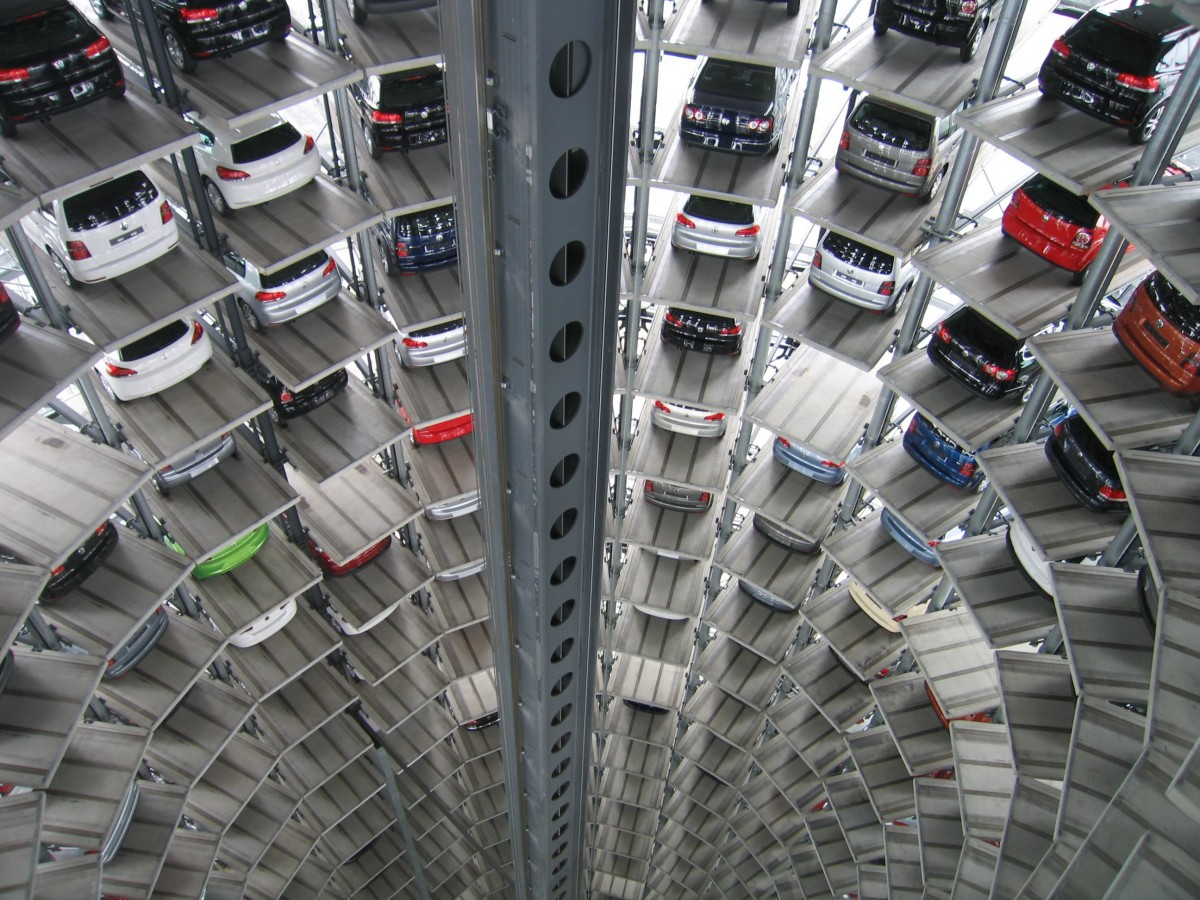
\includegraphics[width=.6\linewidth]{car-tower}}
%\end{frame}

%\subsection{Single System}
%% single-system engineering
%
%\begin{frame}{Greenfield Development? \deutschertitel{Auf der grünen Wiese?}}
%	\href{https://github.com/SoftVarE-Group/SlideTemplate/blob/main/pics/nature/may21-ulm.jpg}{\includegraphics[width=.6\linewidth]{may21-ulm}}
%\end{frame}



% add illustration for variants/versions (space/time) by icons of word/excel/powerpoint/one note/... over the years
